\chapter{Estatística da medida química}\label{ch:b2:measurement-statistics}

Dois laboratórios medem o chumbo da mesma água de torneira e informam 9.6 e \qty{11.2}{\micro g/L}.
O valor-guia para a água potável é \qty{10}{\micro g/L}. A água é própria para beber? Os dois
laboratórios estão mesmo em desacordo, ou os dois resultados são o mesmo valor visto através da
dispersão de duas medidas? Um número vindo de uma análise não significa nada sem sua incerteza, e este
capítulo dá as ferramentas para calculá-la: a estatística das medidas repetidas, a propagação das
incertezas através de um cálculo, a calibração por mínimos quadrados, e os limites abaixo dos quais um
método nada vê.
% ledger: who:lead

\begin{omfigure}
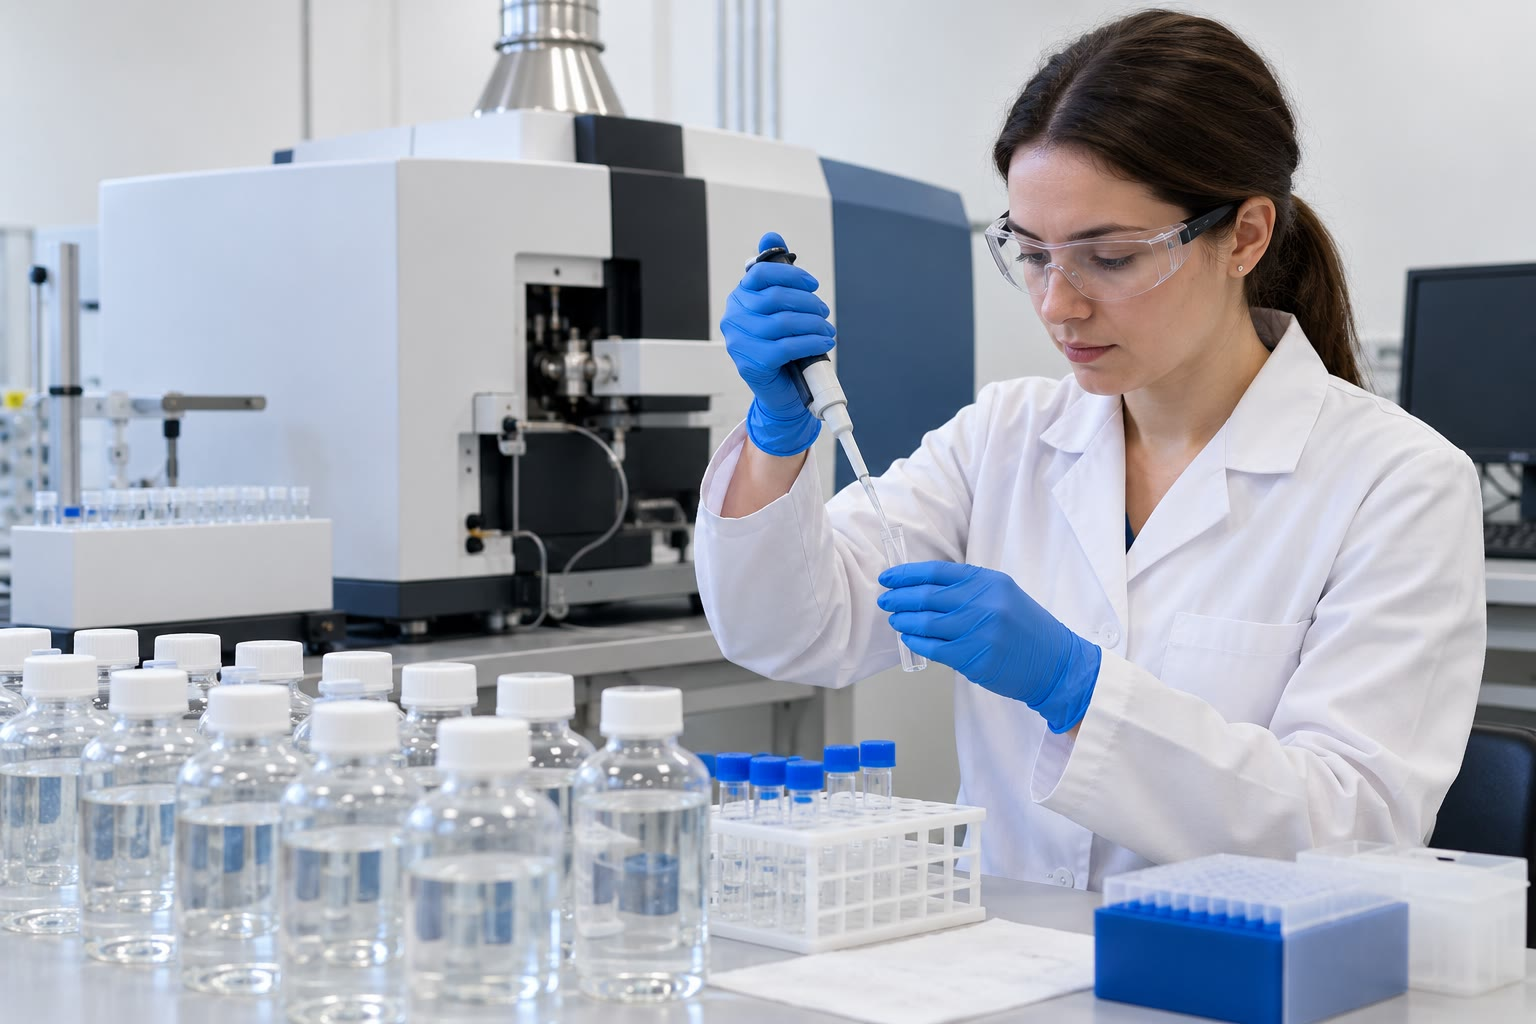
\includegraphics[width=0.56\linewidth]{images/book3/ai/b2-34-water-lab.jpg}

{\small Um laboratório de análise de água: frascos de amostra, um técnico pipetando, um analisador
elementar ao fundo (ilustração).}
\end{omfigure}

\begin{recall}
O volume do 1.º ano: incerteza de medição, incerteza-padrão, avaliações do tipo A e do tipo B,
incerteza expandida, incerteza relativa, o desvio normalizado $z$ entre dois valores, e a promessa de
uma demonstração de $u(\bar x) = s/\sqrt n$ e de uma regra geral de propagação. O volume escolar: a
reta de calibração. \Cref{ch:b2:mass-spec-atomic}: a absorção atômica.
\end{recall}

\section{As medidas repetidas}

Repita uma medida e os resultados se dispersam. Tratamos cada resultado $x_i$ como uma variável
aleatória de média $\mu$ (o valor que o método daria em média) e desvio-padrão $\sigma$; quando muitas
pequenas causas independentes se somam, os resultados seguem a lei normal (gaussiana), cerca de 68~\%
deles dentro de $\mu \pm \sigma$ e 95~\% dentro de $\mu \pm 1.96\sigma$.

\begin{definition}[Dispersão]\label{def:b2:measurement-statistics:dispersion}
Para $n$ resultados $x_1, \dots, x_n$ de média $\bar x$, o \emph{desvio-padrão
experimental}\index{desvio-padrao experimental@desvio-padrão experimental} é $s = \sqrt{\sum (x_i - \bar x)^2/(n-1)}$; ele
estima $\sigma$. O \emph{desvio-padrão da média}\index{desvio-padrao da media@desvio-padrão da média} é
o desvio-padrão de $\bar x$ sobre muitas séries de $n$ resultados, estimado por $s/\sqrt n$.
\end{definition}

O divisor $n - 1$ em vez de $n$ corrige o fato de que os desvios são tomados em relação a $\bar x$,
calculado ele próprio a partir dos mesmos dados, o que os torna um pouco pequenos demais: $n - 1$ é o
número de desvios independentes, os graus de liberdade.

\begin{theorem}[Variância da média]\label{thm:b2:measurement-statistics:mean-variance}
Se $x_1, \dots, x_n$ são independentes, cada um de variância $\sigma^2$, então $\operatorname{var}(\bar x) =
\sigma^2/n$: o \omterm{def:b2:measurement-statistics:dispersion}{desvio-padrão da média} é $\sigma/\sqrt n$.
\end{theorem}

\begin{proof}
Para variáveis independentes, a variância de uma soma é a soma das variâncias, e
$\operatorname{var}(cX) = c^2\operatorname{var}(X)$. Logo $\operatorname{var}(\bar x) =
\operatorname{var}\bigl(\tfrac1n\sum x_i\bigr) = \tfrac{1}{n^2}\sum\operatorname{var}(x_i) =
\tfrac{1}{n^2}\,n\sigma^2 = \sigma^2/n$. Substituir $\sigma$ por sua estimativa $s$ dá a incerteza-padrão
do tipo A $u(\bar x) = s/\sqrt n$ admitida no volume do 1.º ano.
\end{proof}

\section{Os intervalos de confiança}

\begin{definition}[Intervalo de confiança]\label{def:b2:measurement-statistics:confidence}
Um \emph{intervalo de confiança}\index{intervalo de confianca@intervalo de confiança} com \emph{nível de confiança}\index{nivel de confianca@nível de confiança}
$1 - \alpha$ (muitas vezes 95~\%) é um intervalo calculado a partir dos dados por uma regra que,
aplicada a muitas séries, contém o valor verdadeiro em uma fração $1 - \alpha$ delas. Para a média de
$n$ resultados, ele é $\bar x \pm t\,s/\sqrt n$, onde $t$ é o \emph{coeficiente de Student}\index{coeficiente de Student}
para $n - 1$ graus de liberdade e esse nível.
\end{definition}

\begin{proposition}[Lei de Student]\label{prop:b2:measurement-statistics:student}
Para $n$ resultados normais independentes, $T = (\bar x - \mu)/(s/\sqrt n)$ segue a lei de Student com
$n - 1$ graus de liberdade, cuja densidade é proporcional a $(1 + t^2/\nu)^{-(\nu+1)/2}$ com
$\nu = n - 1$. Ela é mais larga que a lei normal e tende a ela quando $n$ cresce.
\end{proposition}

\admitted

Dividir por $s$ em vez do $\sigma$ desconhecido acrescenta a dispersão do próprio $s$, que é grande
quando $n$ é pequeno; daí as caudas mais pesadas, e coeficientes maiores que 1.96. A tabela dá os
coeficientes a 95~\%, calculados a partir da densidade.

\begin{omfigure}
\begin{minipage}[c]{0.56\linewidth}
\begin{tikzpicture}
\begin{axis}[width=\linewidth, height=4.8cm, xmin=-5, xmax=5, ymin=0, ymax=0.43,
  xlabel={$t$}, ylabel={densidade}, label style={font=\small}, tick label style={font=\scriptsize},
  legend style={font=\scriptsize, at={(0.98,0.98)}, anchor=north east}, legend cell align=left]
\addplot[omThm, thick] table[x=t, y=nu2] {figdata/out/bachelor-2-regression-c.dat};
\addplot[omMeth, thick] table[x=t, y=nu5] {figdata/out/bachelor-2-regression-c.dat};
\addplot[black, thick, dashed] table[x=t, y=normal] {figdata/out/bachelor-2-regression-c.dat};
\legend{$\nu = 2$, $\nu = 5$, normal}
\end{axis}
\end{tikzpicture}
\end{minipage}\hfill
\begin{minipage}[c]{0.4\linewidth}\centering
\small
\begin{tabular}{rr}
\hline
$\nu = n - 1$ & $t$ (95~\%) \\
\hline
1 & 12.706 \\
2 & 4.303 \\
3 & 3.182 \\
4 & 2.776 \\
5 & 2.571 \\
9 & 2.262 \\
20 & 2.086 \\
$\infty$ & 1.960 \\
\hline
\end{tabular}
\end{minipage}
\par\vspace{4pt}

{\small Densidades de Student para 2 e 5 graus de liberdade comparadas à lei normal, e os coeficientes
bilaterais a 95~\%, calculados integrando a densidade (a última linha é a lei normal).}
% figdata: bachelor-2/regression.py parts c, e
\end{omfigure}

\begin{method}[Um intervalo de confiança para uma média]\label{met:b2:measurement-statistics:confidence-interval}
\begin{enumerate}
  \item Calcule $\bar x$ e $s$ dos $n$ resultados; verifique que nenhum resultado está grosseiramente fora.
  \item Leia $t$ para $\nu = n - 1$ no nível escolhido.
  \item Informe $\bar x \pm t\,s/\sqrt n$, com a incerteza arredondada a um ou dois algarismos
        significativos e a média à mesma casa decimal.
  \item Para comparar com um valor de referência $x_{\mathrm{ref}}$, calcule $|\bar x - x_{\mathrm{ref}}|/(s/\sqrt
        n)$: acima de $t$, a diferença é significativa nesse nível; abaixo, os dados não mostram uma
        diferença (o que não prova que não haja nenhuma).
\end{enumerate}
\end{method}

\section{A propagação das incertezas}

\begin{theorem}[Lei de propagação das incertezas]\label{thm:b2:measurement-statistics:propagation}
Se $y = f(x_1, \dots, x_n)$, onde os $x_i$ são independentes, com incertezas-padrão $u(x_i)$ pequenas
o bastante para que $f$ seja quase linear nessa escala, então
\begin{equation*}
u^2(y) = \sum_{i=1}^{n}\left(\frac{\partial f}{\partial x_i}\right)^2 u^2(x_i).
\end{equation*}
\end{theorem}

\begin{proof}
Em primeira ordem (Taylor), $y - f(\mu_1, \dots, \mu_n) \approx \sum c_i(x_i - \mu_i)$ com $c_i = \partial
f/\partial x_i$ nas médias. A variância de uma combinação linear de variáveis independentes é
$\sum c_i^2\operatorname{var}(x_i)$ (como no \cref{thm:b2:measurement-statistics:mean-variance}); com
$\operatorname{var}(x_i) = u^2(x_i)$, este é o resultado.
\end{proof}

\begin{corollary}[Somas e produtos]\label{cor:b2:measurement-statistics:products}
Para uma soma ou uma diferença, as incertezas-padrão se somam em quadratura: $u^2(x_1 \pm x_2) = u^2(x_1) +
u^2(x_2)$. Para um produto ou um quociente $y = x_1^{a}x_2^{b}\cdots$, as incertezas relativas se somam
em quadratura, cada uma ponderada por seu expoente: $\bigl(u(y)/y\bigr)^2 = a^2\bigl(u(x_1)/x_1\bigr)^2 +
b^2\bigl(u(x_2)/x_2\bigr)^2 + \cdots$
\end{corollary}

\begin{proof}
Para uma soma, as derivadas parciais valem $\pm1$. Para $y = x_1^ax_2^b$, $\partial y/\partial x_1 =
a\,y/x_1$ e $\partial y/\partial x_2 = b\,y/x_2$; o teorema dá $u^2(y) = a^2y^2u^2(x_1)/x_1^2 +
b^2y^2u^2(x_2)/x_2^2$; divida por $y^2$.
\end{proof}

\begin{method}[Propagar]\label{met:b2:measurement-statistics:propagate}
\begin{enumerate}
  \item Escreva o resultado como uma fórmula das grandezas medidas; liste cada entrada com sua incerteza
        padrão (tipo A ou B).
  \item Para produtos e quocientes, trabalhe com incertezas relativas; para somas, com as absolutas;
        nos outros casos, tome derivadas parciais.
  \item Combine em quadratura; encontre o termo dominante: melhorar os outros é esforço perdido.
  \item Multiplique pelo fator de abrangência (2, ou o $t$ de Student quando o termo dominante vem de
        poucas repetições) para obter uma incerteza expandida.
\end{enumerate}
\end{method}

\section{A calibração}

\begin{definition}[Curva de calibração]\label{def:b2:measurement-statistics:calibration}
Uma \emph{curva de calibração}\index{curva de calibracao@curva de calibração} relaciona o sinal $y$ de um instrumento à
concentração $x$, a partir de padrões de concentração conhecida. A \emph{reta dos mínimos
quadrados}\index{reta dos minimos quadrados@reta dos mínimos quadrados} $y = a + bx$ é a reta que minimiza $S = \sum (y_i - a -
bx_i)^2$; cada $e_i = y_i - a - bx_i$ é um \emph{resíduo}\index{residuo@resíduo}.
\end{definition}

\begin{theorem}[Reta dos mínimos quadrados]\label{thm:b2:measurement-statistics:least-squares}
Com $\bar x$, $\bar y$ as médias, $S_{xx} = \sum(x_i - \bar x)^2$ e $S_{xy} = \sum(x_i - \bar x)(y_i -
\bar y)$, a \omterm{def:b2:measurement-statistics:calibration}{reta dos mínimos quadrados} tem
\begin{equation*}
b = \frac{S_{xy}}{S_{xx}}, \qquad a = \bar y - b\bar x.
\end{equation*}
\end{theorem}

\begin{proof}
$S$ é uma função quadrática de $a$ e $b$. Suas derivadas parciais se anulam no mínimo:
$\partial S/\partial a = -2\sum(y_i - a - bx_i) = 0$ dá $a = \bar y - b\bar x$; substituindo em
$\partial S/\partial b = -2\sum x_i(y_i - a - bx_i) = 0$ obtém-se $\sum x_i\bigl((y_i - \bar y) - b(x_i -
\bar x)\bigr) = 0$, isto é, $S_{xy} = bS_{xx}$ (pois $\sum \bar x(y_i - \bar y) = \sum \bar x(x_i - \bar
x) = 0$). As derivadas segundas formam a matriz
\[\begin{pmatrix} 2n & 2\sum x_i\\ 2\sum x_i & 2\sum x_i^2\end{pmatrix},\]
cuja diagonal é positiva e cujo determinante $4nS_{xx}$ é positivo quando os $x_i$ não são todos
iguais: o ponto estacionário é um mínimo.
\end{proof}

\begin{proposition}[Ler uma concentração]\label{prop:b2:measurement-statistics:interpolation}
Para $n$ padrões com desvio-padrão residual $s_{y/x} = \sqrt{\sum e_i^2/(n-2)}$, uma amostra lida
$m$ vezes com sinal médio $\bar y_0$ tem $x_0 = (\bar y_0 - a)/b$ e desvio-padrão
\begin{equation*}
s_{x_0} = \frac{s_{y/x}}{b}\sqrt{\frac1m + \frac1n + \frac{(\bar y_0 - \bar y)^2}{b^2S_{xx}}},
\end{equation*}
a ser usado com o $t$ de Student para $n - 2$ graus de liberdade.
\end{proposition}

\admitted

Os três termos sob a raiz são a dispersão das leituras da amostra, a incerteza da altura da reta e a
de sua inclinação; o último se anula no centro da faixa de calibração, que é onde as amostras são mais
bem lidas.

\begin{omfigure}
\begin{tikzpicture}
\begin{axis}[width=0.5\linewidth, height=5cm, xmin=-1, xmax=22, ymin=0, ymax=0.22,
  xlabel={chumbo (\unit{\micro g/L})}, ylabel={absorbância}, label style={font=\small},
  tick label style={font=\scriptsize}, scaled y ticks=false,
  yticklabel style={/pgf/number format/fixed, /pgf/number format/precision=2}]
\addplot[omDef, thick] table[x=x, y=line] {figdata/out/bachelor-2-regression-b.dat};
\addplot[only marks, mark=*, mark size=1.8pt, omThm] table[x=x, y=A] {figdata/out/bachelor-2-regression-a.dat};
\end{axis}
\end{tikzpicture}\hfill
\begin{tikzpicture}
\begin{axis}[width=0.5\linewidth, height=5cm, xmin=-1, xmax=22, ymin=-0.002, ymax=0.002,
  xlabel={chumbo (\unit{\micro g/L})}, ylabel={resíduo}, label style={font=\small},
  tick label style={font=\scriptsize}, scaled y ticks=false, ycomb,
  yticklabel style={/pgf/number format/fixed, /pgf/number format/precision=3},
  extra y ticks={0}, extra y tick style={grid=major, grid style={black!50}}]
\addplot[omThm, thick, mark=*, mark size=1.6pt] table[x=x, y=res] {figdata/out/bachelor-2-regression-a.dat};
\end{axis}
\end{tikzpicture}

{\small Calibração do chumbo por absorção atômica em forno de grafite a \qty{283.3}{nm} (dados do
exercício, usados no problema). À esquerda: os cinco padrões e a \omterm{def:b2:measurement-statistics:calibration}{reta dos mínimos quadrados}. À direita:
os \omterm{def:b2:measurement-statistics:calibration}{resíduos}, pequenos e sem padrão: uma reta é adequada.}
% figdata: bachelor-2/regression.py parts a, b
% ledger: asd:Pb283
\end{omfigure}

\begin{method}[Calibrar]\label{met:b2:measurement-statistics:calibrate}
\begin{enumerate}
  \item Prepare cinco padrões ou mais que cubram a faixa esperada, na mesma matriz que as amostras,
        e um branco.
  \item Ajuste a \omterm{def:b2:measurement-statistics:calibration}{reta dos mínimos quadrados}; trace os \omterm{def:b2:measurement-statistics:calibration}{resíduos}. Um padrão curvo significa que a resposta
        não é linear: estreite a faixa ou ajuste uma curva. Um \omterm{def:b2:measurement-statistics:calibration}{resíduo} grande isolado aponta para um
        padrão defeituoso.
  \item Leia as amostras, de preferência perto do meio da faixa, em réplicas; calcule $x_0$ e
        $s_{x_0}$.
  \item Informe $x_0 \pm t\,s_{x_0}$ após corrigir cada diluição, acrescentando a incerteza propagada
        da diluição se ela não for desprezível.
\end{enumerate}
\end{method}

\begin{definition}[Adição padrão]\label{def:b2:measurement-statistics:standard-addition}
No \emph{método da adição padrão}\index{metodo da adicao padrao@método da adição padrão}, quantidades conhecidas de analito são
acrescentadas a porções iguais da própria amostra; o sinal é traçado em função da concentração
acrescentada, e a concentração do analito na amostra é a distância da origem ao ponto em que a reta
extrapolada até o sinal nulo corta o eixo, $a/b$.
\end{definition}

\begin{method}[Adição padrão]\label{met:b2:measurement-statistics:standard-addition}
\begin{enumerate}
  \item Use-a quando a matriz da amostra muda a resposta (sais, ácidos, matéria orgânica), de modo que
        padrões em água pura dariam uma inclinação errada.
  \item Dope porções iguais com quantidades conhecidas crescentes, dilua todas ao mesmo volume, meça.
  \item Ajuste a reta; a concentração nas soluções medidas é $a/b$; corrija a diluição.
  \item A resposta deve ser linear desde zero: verifique os \omterm{def:b2:measurement-statistics:calibration}{resíduos}.
\end{enumerate}
\end{method}

\begin{omfigure}
\begin{tikzpicture}
\begin{axis}[width=0.62\linewidth, height=5cm, xmin=-4, xmax=7, ymin=0, ymax=0.42,
  xlabel={concentração acrescentada (\unit{mg/L})}, ylabel={absorbância}, label style={font=\small},
  tick label style={font=\scriptsize}, axis lines=left, scaled y ticks=false,
  yticklabel style={/pgf/number format/fixed, /pgf/number format/precision=1}]
\draw[black!40] (axis cs:0,0) -- (axis cs:0,0.42);
\addplot[omDef, thick, densely dashed] table[x=x, y=line] {figdata/out/bachelor-2-regression-d-line.dat};
\addplot[only marks, mark=*, mark size=1.8pt, omThm] table[x=x, y=A] {figdata/out/bachelor-2-regression-d.dat};
\draw[<->, omMeth, thick] (axis cs:-3.11,0.06) -- (axis cs:0,0.06); \node[omMeth, below, font=\scriptsize] at (axis cs:-0.8,0.055) {$a/b$};
\end{axis}
\end{tikzpicture}

{\small Adição padrão (dados do exercício): absorbância de uma amostra dopada com 0, 2, 4 e
\qty{6}{mg/L} de analito. A reta encontra o sinal nulo em \qty{-3.11}{mg/L}: a solução medida
continha \qty{3.11}{mg/L}.}
% figdata: bachelor-2/regression.py part d
\end{omfigure}

\section{Detecção, quantificação e validação}

\begin{definition}[Limites]\label{def:b2:measurement-statistics:limits}
O \emph{limite de detecção}\index{limite de deteccao@limite de detecção} de um método é a menor concentração cujo
sinal pode ser distinguido do de um branco com um pequeno risco declarado de falsa detecção; o
\emph{limite de quantificação}\index{limite de quantificacao@limite de quantificação} é a menor concentração que pode
ser medida com uma incerteza relativa aceitável.
\end{definition}

\begin{proposition}[Estimativas usuais]\label{prop:b2:measurement-statistics:lod}
Com $s_{\mathrm{branco}}$ o desvio-padrão de sinais de branco repetidos e $b$ a inclinação da
reta de calibração, $x_{\mathrm{LD}} \approx 3s_{\mathrm{branco}}/b$ e $x_{\mathrm{LQ}} \approx
10s_{\mathrm{branco}}/b$.
\end{proposition}

\begin{proof}[Raciocínio]
Se os sinais de branco são normais com desvio-padrão $s_{\mathrm{branco}}$, um branco excede sua média
em mais de $3s_{\mathrm{branco}}$ com probabilidade de cerca de 0.13~\% (cauda unilateral da lei normal
além de 3 desvios-padrão): declarar ``detectado'' um sinal acima desse limiar raramente confunde um
branco com uma amostra. Um sinal $10s_{\mathrm{branco}}$ acima do branco tem um desvio-padrão relativo de
cerca de 10~\%, o limiar habitual para um resultado quantitativo. Dividir por $b$ converte sinais em
concentrações.
\end{proof}

\begin{definition}[Validação]\label{def:b2:measurement-statistics:validation}
A \emph{veracidade}\index{veracidade} é a proximidade entre a média de um grande número de resultados e o valor
verdadeiro; sua diferença é o \emph{viés}\index{vies@viés}. A \emph{precisão}\index{precisao@precisão} é a
proximidade entre resultados independentes, expressa como um desvio-padrão:
\emph{repetibilidade}\index{repetibilidade} nas mesmas condições (mesmo operador, instrumento,
laboratório, curto intervalo de tempo), \emph{reprodutibilidade}\index{reprodutibilidade} em condições
alteradas (laboratórios diferentes). A \emph{validação de método}\index{validacao de metodo@validação de método} é o conjunto
de experimentos que estabelecem, para um método, sua veracidade, sua precisão, sua linearidade e sua
faixa, e seus \omterm{def:b2:measurement-statistics:limits}{limites de detecção} e de quantificação.
\end{definition}

A \omterm{def:b2:measurement-statistics:validation}{veracidade} é verificada com um material de referência certificado ou por dopagem; a \omterm{def:b2:measurement-statistics:validation}{precisão}, por
réplicas em um laboratório e por comparações entre laboratórios. Um método pode ser preciso mas
enviesado, cada resultado próximo dos outros e todos eles errados: a \omterm{def:b2:measurement-statistics:validation}{precisão} não prova a \omterm{def:b2:measurement-statistics:validation}{veracidade}.

\begin{history}[Student, 1908]
\begin{minipage}[t]{0.17\linewidth}
\vspace{0pt}
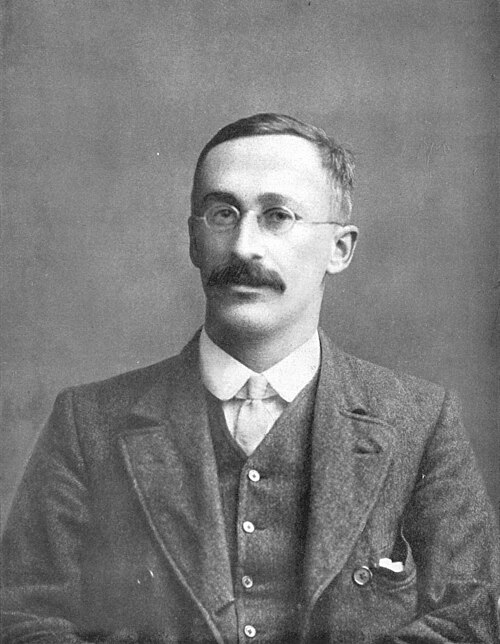
\includegraphics[width=\linewidth]{images/book3/gosset.jpg}
\end{minipage}\hfill
\begin{minipage}[t]{0.79\linewidth}
\vspace{0pt}
William Sealy Gosset, químico de uma cervejaria, tinha de julgar matérias-primas a partir de muito
poucas amostras, poucas demais para a lei normal. Em 1908 ele publicou a distribuição da média dividida
pelo desvio-padrão amostral, sob o pseudônimo ``Student'', porque seu empregador não permitia que os
funcionários publicassem com seus nomes. A lei de Student é usada cada vez que um analista dá um
intervalo a partir de três ou quatro réplicas. (Fotografia, 1908: domínio público; Wikimedia Commons.)
\end{minipage}
\end{history}

\section{Exercícios}

\begin{exercise}[$\star$]\label{exo:b2:measurement-statistics:1}
Cinco titulações dão 12.45, 12.50, 12.48, 12.52 e \qty{12.46}{mL}. Calcule a média, o \omterm{def:b2:measurement-statistics:dispersion}{desvio-padrão
experimental} e o \omterm{def:b2:measurement-statistics:dispersion}{desvio-padrão da média}.
\end{exercise}

\begin{exercise}[$\star$]\label{exo:b2:measurement-statistics:2}
Dê o \omterm{def:b2:measurement-statistics:confidence}{intervalo de confiança} a 95~\% da média do exercício~1.
\end{exercise}

\begin{exercise}[$\star$]\label{exo:b2:measurement-statistics:3}
Uma solução é preparada dissolvendo $m = \qty{0.5000}{g}$ ($u = \qty{0.0002}{g}$) de um sólido em um balão
de $V = \qty{250.0}{mL}$ ($u = \qty{0.15}{mL}$). Calcule a incerteza-padrão relativa de $c = m/(MV)$,
sendo a massa molar suficientemente exata.
\end{exercise}

\begin{exercise}[$\star$]\label{exo:b2:measurement-statistics:4}
Ajuste a \omterm{def:b2:measurement-statistics:calibration}{reta dos mínimos quadrados} que passa por $(0, 0.02)$, $(1, 0.21)$, $(2, 0.39)$, $(3, 0.62)$.
\end{exercise}

\begin{exercise}[$\star\star$]\label{exo:b2:measurement-statistics:5}
Uma solução de referência certificada contém \qty{10.00}{mg/L} de um elemento. Cinco análises dão uma
média de \qty{10.12}{mg/L} com $s = \qty{0.08}{mg/L}$. O método é enviesado no nível de 95~\%?
\end{exercise}

\begin{exercise}[$\star\star$]\label{exo:b2:measurement-statistics:6}
Uma concentração de íons hidrônio é conhecida com uma incerteza-padrão relativa de 2~\%. Qual é a
incerteza-padrão do pH?
\end{exercise}

\begin{exercise}[$\star\star$]\label{exo:b2:measurement-statistics:7}
Dez brancos têm $s = 0.0012$ unidade de absorbância; a inclinação de calibração é \qty{0.0098}{L/\micro g}.
Estime os \omterm{def:b2:measurement-statistics:limits}{limites de detecção} e de quantificação.
\end{exercise}

\begin{exercise}[$\star\star$]\label{exo:b2:measurement-statistics:8}
Na experiência de adição padrão da figura, as quatro porções tinham sido preparadas diluindo
\qty{10.0}{mL} de amostra a \qty{50.0}{mL}. Dê a concentração na amostra.
\end{exercise}

\begin{exercise}[$\star\star$]\label{exo:b2:measurement-statistics:9}
Em um estudo interlaboratorial, cada laboratório obtém $s = \qty{0.05}{mg/L}$ em suas próprias réplicas,
mas os resultados dos diferentes laboratórios se dispersam com $s = \qty{0.15}{mg/L}$. Dê o nome das duas
grandezas e explique a diferença.
\end{exercise}

\begin{exercise}[$\star\star\star$]\label{exo:b2:measurement-statistics:10}
Mostre que a \omterm{def:b2:measurement-statistics:calibration}{reta dos mínimos quadrados} passa por $(\bar x, \bar y)$ e que a soma de seus \omterm{def:b2:measurement-statistics:calibration}{resíduos} é nula.
\end{exercise}

\begin{exercise}[$\star\star\star$]\label{exo:b2:measurement-statistics:11}
Uma solução-estoque é diluída cem vezes, seja em uma etapa (\qty{1.000}{mL} em \qty{100.0}{mL}), seja
em duas etapas de dez vezes (\qty{10.00}{mL} em \qty{100.0}{mL}, duas vezes). Incertezas-padrão: pipeta
de 1 mL \qty{0.006}{mL}, pipeta de 10 mL \qty{0.02}{mL}, balão de 100 mL \qty{0.08}{mL} (dados do
exercício). Que via é mais precisa?
\end{exercise}

\begin{exercise}[$\star\star\star$]\label{exo:b2:measurement-statistics:12}
Os dois laboratórios da introdução informam 9.6 e \qty{11.2}{\micro g/L} com incertezas-padrão
0.4 e \qty{0.5}{\micro g/L} (dados do exercício). Seus resultados são compatíveis? O que cada um diz em
relação ao valor-guia?
\end{exercise}

\section{Problema: O chumbo da água de torneira}

\begin{problem}[{Problema de fim de semana --- uma calibração de absorção atômica por mínimos quadrados,
a concentração de uma amostra com seu intervalo de confiança, a diluição e os limites, e um veredicto
em relação ao valor-guia}]
\label{pb:b2:measurement-statistics:1}
Dados do exercício. O chumbo é medido por absorção atômica em forno de grafite a \qty{283.3}{nm}. Padrões
(\unit{\micro g/L}; absorbância): 0.0; 0.003, 5.0; 0.051, 10.0; 0.101, 15.0; 0.148, 20.0; 0.199. A
água de torneira (\qty{50.0}{mL}) é acidificada com \qty{0.50}{mL} de ácido nítrico; três leituras dessa
solução dão 0.104, 0.098 e 0.101. Dez brancos: 0.002, 0.004, 0.003, 0.001, 0.003, 0.005, 0.002,
0.003, 0.004, 0.003. Incertezas-padrão dos volumes: \qty{0.03}{mL} para 50.0 mL,
\qty{0.005}{mL} para 0.50 mL. Valor-guia: \qty{10}{\micro g/L}.
% ledger: who:lead, asd:Pb283

\medskip
\noindent\textbf{Parte I --- Calibração.}
\begin{enumerate}
  \item Por que os padrões são preparados no mesmo ácido nítrico que as amostras?
  \item Calcule a inclinação e o intercepto da \omterm{def:b2:measurement-statistics:calibration}{reta dos mínimos quadrados}.
  \item Calcule os cinco \omterm{def:b2:measurement-statistics:calibration}{resíduos}.
  \item Os \omterm{def:b2:measurement-statistics:calibration}{resíduos} mostram um padrão? Conclua sobre a linearidade.
  \item Calcule $s_{y/x}$.
  \item Por que o intercepto não é nulo?
  \item O que mede a inclinação?
\end{enumerate}

\medskip
\noindent\textbf{Parte II --- A amostra.}
\begin{enumerate}[resume]
  \item Calcule a média e o desvio-padrão das três leituras.
  \item Calcule a concentração de chumbo da solução medida.
  \item Calcule $s_{x_0}$.
  \item Quantos graus de liberdade, e que \omterm{def:b2:measurement-statistics:confidence}{coeficiente de Student}?
  \item Dê o intervalo a 95~\% da concentração na solução medida.
  \item Por que ler a amostra três vezes em vez de uma?
\end{enumerate}

\medskip
\noindent\textbf{Parte III --- Diluição e limites.}
\begin{enumerate}[resume]
  \item Calcule o fator de diluição e a concentração na água de torneira.
  \item Propague a incerteza dos dois volumes para o fator de diluição.
  \item Essa incerteza é significativa ao lado da incerteza de calibração?
  \item Calcule o desvio-padrão dos brancos e o \omterm{def:b2:measurement-statistics:limits}{limite de detecção}.
  \item Calcule o \omterm{def:b2:measurement-statistics:limits}{limite de quantificação}.
  \item A amostra está acima do \omterm{def:b2:measurement-statistics:limits}{limite de quantificação}?
\end{enumerate}

\medskip
\noindent\textbf{Parte IV --- Veredicto.}
\begin{enumerate}[resume]
  \item O intervalo contém o valor-guia?
  \item O que uma única leitura de 0.104 teria sugerido?
  \item O que significa aqui ``95~\% de confiança''?
  \item Como o laboratório poderia decidir com mais firmeza?
  \item Como ele verificaria que o método não é enviesado?
  \item O valor-guia é provisório ``com base no desempenho do tratamento e na exequibilidade
        analítica''. O que significa a segunda razão, à luz deste problema?
  \item Dê a concentração de chumbo da água de torneira com seu intervalo a 95~\%, e compare-a com
        \qty{10}{\micro g/L}.
\end{enumerate}
\end{problem}
